% !TEX root = ../../document.tex

\documentclass{subfiles}

\begin{document}

  \chapter{Formulación del Problema}
  \label{chap:formulation}

    \section{Introducción}
    \label{sec:formulation_introduction}

      \paragraph{}
      El problema \emph{Dial-a-Ride} (o \emph{DARP} en modo abreviado) representa una de las modelizaciones más interesantes en el ámbito de los problemas de \emph{optimización combinatoria}. Esto se debe a la gran cantidad de situaciones del mundo real que pueden ser representadas siguiendo dicho esquema. Sin embargo, antes de profundizar en los aspectos más detallados que caracterizan este modelo, es necesario describir el contexto del mismo así como la clase problemas a la cual pertenece. Una vez se haya completado dicha tarea, se estará en condiciones suficientes para poder describir tanto la versión básica como las extensiones más interesantes, tando desde el punto de vista de los aspectos matemáticos, como desde la cantidad de situaciones reales que permiten resolver.

      \paragraph{}
      En los últimos años, el número de compañias que basan su modelo de negocio en alguna variante relacionada con el problema \emph{Dial-a-Ride} ha crecido de manera desmesurada. Algunos ejemplos son aquellas basadas en el reparto de comida (u otros productos) desde los establecimientos hasta la casa de los solicitantes, o la modernización del sector del transporte privado en ciudad gracias a la solicitud de viajes desde el dispositivo móvil. Es importante darse cuenta de que dichas compañías llevan a cabo la planificación en tiempo real ya que en contadas ocasiones los clientes solicitan sus servicios con demasiada antelación. Sin embargo, para poder desarrollar soluciones interesantes sobre entornos en tiempo real, lo primero es poder comprender el problema de manera detallada en su versión estática, para después poder llevar a cabo las simplificaciones y extensiones pertinentes que permiten la toma de decisiones de manera eficiente en entornos dinámicos. Por tanto, este capítulo se centra especialmente en la descripción del modelo estático. 

      \paragraph{}
      En cuanto a la organización del capítulo, en el \cref{sec:formulation_contextualization} se describe de manera detallada el problema \emph{Dial-a-Ride} desde el punto de vista de la jerarquía de clases a la cual pertenecen siguiendo un enfoque descendente (o \emph{top-down}) en los \cref{sec:formulation_optimization_problems,sec:formulation_linear_problems,sec:formulation_combinatorial_problems,sec:formulation_generalized_pickup_and_delivery_problems,sec:formulation_routing_pickup_and_delivery_problems,sec:formulation_dial_a_ride_problems}. Seguidamente, en el apartado \cref{sec:formulation_notation} se indica la notación que se pretende seguir a lo largo del documento (y que pretende ser utilizada a modo de referencia en capítulos posteriores). El siguiente paso es determinar la \emph{Formulación Básica}, lo cual se lleva a cabo en el \cref{sec:formulation_basic_formulation}. Finalmente, en el \cref{sec:formulation_conclusions} se describen brevemente los aspectos más importantes del capítulo.

    \section{Contextualización del problema}
    \label{sec:formulation_contextualization}

      \paragraph{}
      A continuación se procede a describir la clase de problemas matemáticos a la cual pertenece el problema \emph{Dial-a-Ride}. Dicha descripción se llevará a cabo de fuera hacia dentro, esto es desde la categoría de problemas más amplia hasta la más concreta, pasando por una breve contextualización así como ejemplificación de problemas similares. En la \cref{img:formulation_dial_a_ride_contextualization} se muestra un breve resumen gráfico acerca de las clases de problemas que se describen.

      \begin{figure}[ht]
        \centering
        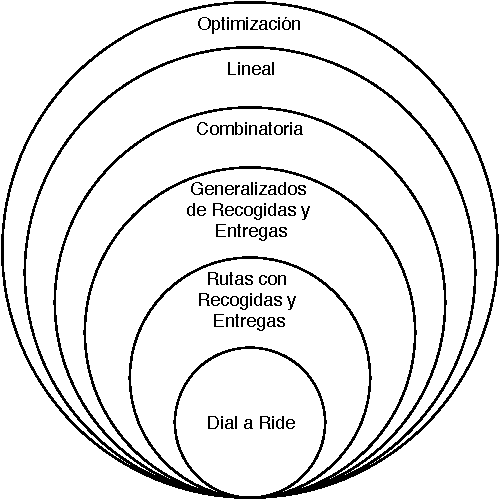
\includegraphics[width=0.4\textwidth]{dial_a_ride_context}
        \caption{Contextualización del \emph{Problema Dial-a-Ride} desde el punto de vista de la jerarquía de problemas a la que pertenece.}
        \label{img:formulation_dial_a_ride_contextualization}
      \end{figure}

      \subsection{Problemas de Optimización}
      \label{sec:formulation_optimization_problems}

        \paragraph{}
        La clase de \emph{problemas de optimización} representa una de las áreas de investigación más interesante en la actualidad, ya que muchas de las innovaciones obtenidas en dicho campo permiten resolver problemas aplicables al mundo real de manera práctica que antes únicamente podían ser resueltos teóricamente. En concreto, los problemas de optimización son aquellos que se basan en la minimización (o maximización) de una determinada función objetivo (posiblemente vectorial, lo cual define modelos multiobjetivo) de manera que se satisfaga un conjunto de restricciones previamente fijadas sobre un conjunto de variables de decisión que afectan mutuamente a la satisfacibilidad de las restricciones y el valor de la función objetivo.

        \paragraph{}
        Dichas variables de decisión pueden ser tanto categóricas como numéricas (discretas o continuas), lo cual genera una gran cantidad de subproblemas diferences (Nótese que las variables categóricas con $k$ niveles diferentes pueden ser representadas de manera sencilla a partir de $k-1$ variables binarias). De la misma manera, tanto el valor de función objetivo como las restricciones pueden tener una naturaleza muy diferente: estas pueden estar formadas por funciones lineales de las variables de decisión, como por complicadas funciones no lineales que complican el proceso de obtención del valor óptimo del problema. De manera matemática, la \cref{eq:general_optimization_formulation} define la formulación de optimización, donde tanto las funciones $f_i(\cdot)$ como $g_k(\cdot)$ son funciones arbitrarias que proyectan el vector de variables de decisión $n$-dimensional $\mathbf{x}$ en un espacio unidimensional (generando un valor escalar).

        \begin{eqfloat}
          \begin{equation}
            \begin{array}{rr@{}ll}
              \underset{\mathbf{x} \in \mathbb{R}^{n}}{\text{Minimizar}} & f_i(\mathbf{x}) &                 ,& \forall i \in \{1,...,I\} \\
              \text{sujeto a}	 & g_k(\mathbf{x}) \ &\leq 0, & \forall k \in \{1,...,K\}
            \end{array}
          \end{equation}
          \caption{Formulación del modelo de Optimización General}
          \label{eq:general_optimization_formulation}
        \end{eqfloat}

        \paragraph{}
        Muchos de los problemas que resolvemos a diario en nuestra vida cotidiana son en cierta medida \emph{problemas de optimización}, desde qué elementos decidimos añadir a nuestra mochila cada día (basados en restricciones de capacidad, funciones objetivo de utilidad y variables de decisión binarias) hasta el la detección del rostro por nuestros teléfonos móviles para aplicar un filtro de la manera más realista posible en una videollamada (basados en restricciones de forma, funciones objetivo multidimensionales y millones de variables de decisión numéricas).

      \subsection{Problemas de Optimización Lineal}
      \label{sec:formulation_linear_problems}

        \paragraph{}
        Una de las categorías de problemas de optimización más ampliamente estudiados por su relativa simplicidad (ya se han desarrollado métodos capaces de obtener soluciones óptimas en un número reducido de pasos) y su gran capacidad de modelización ante muchas situaciones del mundo real son los \emph{problemas de optimización lineal}. Dichos problemas se caracterizan por estar compuestos por variables de decisión compuestas por transformaciones lineales respecto de la función objetivo. Esto quiere decir que tanto el valor de la función objetivo como las posibles restricciones escritas en forma de desigualdades están compuestas por sumas de las variables de decisión multiplicadas por determinados pesos.

        \paragraph{}
        En la \cref{eq:linear_optimization_formulation} se muestra a modo de ejemplo la formulación de un problema de optimización lineal (del cual se hablará posteriormente). Como se puede apreciar, en este caso las funciones arbitrarias definidas en la formulación general han sido sustituidas por transformaciones lineales respecto de las variables de decisión. Para la resolución de problemas de este tipo se han desarrollado una gran cantidad de métodos, entre los que destaca un algoritmo altamente eficiente el cual se conoce como \emph{Simplex} \cite{klee1970good}. Este algoritmo se basa en pivotaje entre soluciones de manera que tras cada iteracción se llegue a una solución igual o mejor. Una de las mayores ventajas de la formulación de un problema como lineal es que algoritmos como \emph{Simplex} proporcionan garantias de optimalidad al alcanzar el valor óptimo al terminar completamente su ejecución.

        \begin{eqfloat}
          \begin{equation}
            \begin{array}{rr@{}ll}
              \text{Minimizar} & \sum\limits_{i = 1}^{N}\sum\limits_{j = 1}^{M}  c_{ij}x_{ij} &                 & \\
              \text{sujeto a}	 & \sum\limits_{i = 1}^{N} x_{ij} \ &= s_{i}, & \forall i \in \{1,...,N\} \\
                               & \sum\limits_{j = 1}^{M} x_{ij} \ &= d_{j}, & \forall j \in \{1,...,M\} \\
                               &                               	x_{ij} 	&\geq 0, 	                 & \forall i \in \{1,...,N\},\forall j \in \{1,...,M\}
            \end{array}
          \end{equation}
          \caption{Formulación de un modelo de \emph{Optimización Lineal}. En concreto, el \emph{Problema de Transporte}.}
          \label{eq:linear_optimization_formulation}
        \end{eqfloat}

        \paragraph{}
        A pesar de que el algoritmo \emph{Simplex} siempre proporcione resultados óptimos, en algunas ocasiones no se posee la capacidad suficiente de cálculo para llegar a la mejor solución. Por lo tanto, se han desarrollado una gran cantidad de métodos conocidos como \emph{heurísticos} (de los cuáles se hablará más en detalle en el los \cref{sec:solving_heuristics,sec:solving_metaheuristics}) que a pesar de proporcionar unos buenos resultados, no ofrecen ninguna garantia de optimalidad. Por contra, también existen otros métodos exactos que son capaces de llegar al valor óptimo utilizando menor cantidad de recursos (algunos de los cuales se describen en el \cref{sec:solving_exacts}).

        \paragraph{}
        Antes de describir algunos de los ejemplos y aplicaciones reales más destacadas basadas en \emph{problemas de optimización lineal}, es necesario describir unos de los problemas más populares de esta categoria, el cual se conoce como \emph{problema de transporte} y se caracteriza por permitir representar de manera matemática la tarea sobre cómo distribuir un conjunto de recursos procedentes de $N$ puntos de origen hasta $M$ puntos de destino, donde cada trayecto tiene un coste diferente, y cada origen y destino unas capacidades de oferta y demanda. La formulación sobre dicho problema se corresponde con la utilizada a modo de ejemplo en la \cref{eq:linear_optimization_formulation}.

        \paragraph{}
        Sin embargo, los problemas de optimización lineal permiten representar una amplia cantidad de situaciones de nuestra vida diaria. Entre ellos se encuentran los \emph{problemas de mezclas} (donde se pretende generar un compuesto con unas ciertas características a partir de la combinación de otros tratando de reducir los costes) aunque los problemas de optimización lineal también son de gran utilidad en el ámbito de la economia y los estudios de mercado, permitiendo representar de una manera relativamente sencilla el comportamiento de los clientes ante cambios de precio u otras variables más elaboradas.

      \subsection{Problemas de Optimización Combinatoria}
      \label{sec:formulation_combinatorial_problems}

        \paragraph{}
        Uno de los factores más relevantes cuando se trata de \emph{problemas de optimización lineal} se refiere a l naturaleza de las variables de decisión, en que (como se ha comentado anteriormente) estas pueden ser de una naturaleza continua o discreta. En este sentido, los problemas pueden clasificarse en 4 categorías: problemas de optimización continua puros (donde existen métodos muy eficientes que permiten ser resueltos en un tiempo razonable), problemas de \emph{optimización entera}, problemas de optimización binaria (o de \emph{optimización combinatoria}) y problema de optimización mixtos (donde mezclan ambos tipos de variables). Para profundizar más en el tema de la \emph{optimización entera} y \emph{optimización combinatoria} se recomienda \cite{wolsey2014integer}

        \paragraph{}
        A pesar de que la exigencia de que las variables de decisión sean discretas en un primer momento puede parecer muy sencilla en un primer momento (por ser muy intuitiva a nivel conceptual), esta complica mucho la labor de optimización del problema. En modo abstracto, esto se debe a que si el espacio de soluciones de un problema de optimización lineal era visto como un prima en un espacio $n$-dimensional (donde $n$ es el número de variables de decisión) y los puntos de interés se refieren a los vértices, que presentarán el máximo/mínimo valor óptimo, en el caso de las variables discretas el prima se transforma en una estructura \say{pixelada} lo cual incrementa de manera exponencial el número de vértices (y por tanto de puntos de evaluación) del problema en la búsqueda del valor óptimo.

        \paragraph{}
        Las dificultades descritas en el párrafo anterior provocan que la clase de problemas de optimización de variables discretas, entre los que se encuentra la de los problemas de optimización combinatoria (a la cuál a su vez pertenecen los de rutas, de los que se hablará posterirmente), hacen que el espacio de soluciones se extienda de tal manera que para casos relativamente pequeños, este sea inabordable. A pesar de existir métodos exactos (de los cuales se hablará en el \cref{sec:solving_exacts}), la mayor parte de la literatura sobre este tema se ha dedicado a la investigación de métodos que a pesar de no ofrecer garantías de optimalidad, proporcionan un buen acuerdo entre eficiencia computacional y calidad de las soluciones obtenidas (los cuales se detallan en los \cref{sec:solving_heuristics,sec:solving_metaheuristics}).

        \begin{eqfloat}
          \begin{equation}
            \begin{array}{rr@{}ll}
              \text{Maximizar} & \sum\limits_{i = 1}^{N} u_{i}x_{i} &                 & \\
              \text{sujeto a}	 & \sum\limits_{i = 1}^{N} w_{i}x_{i} \ &\leq W, & \forall i \in \{1,...,N\} \\
                               &                             	x_{i} 	&\in \{0, 1\}, 	                 & \forall i \in \{1,...,N\}
            \end{array}
          \end{equation}
          \caption{Formulación de un modelo de \emph{Optimización Combinatoria}. En concreto, el \emph{Problema de la Mochila}.}
          \label{eq:combinatorial_optimization_formulation}
        \end{eqfloat}

        \paragraph{}
        Los problemas de \emph{optimización combinatatoria} se caracterizan porque las variables de decisión del modelo son de caracter binario. Dicha razón permite representar situaciones muy interesantes y diversas del mundo real, lo cual ha hecho que los campos de aplicaciones de este tipo de problemas sean desde la generación de rutas de vehículos con garantías de conectividad, hasta problemas de decisión relacionados con la toma o no de una determinada acción. Dentro de los problemas de decisión, existe uno que destaca sobre el resto por su relativa simplicidad teórica, pero a la vez extremada practicidad, el cual se conoce como \emph{problema de la mochila}. A pesar de tener muchas vertientes y extensiones, la idea básica de este es la de maximizar el valor en el proceso de selección de un subconjunto de elementos, dadas unas limitaciones de capacidad y un valor determinado para cada producto. La \say{dificultad} de este modelo reside en que los elementos no pueden ser escogidos parcialmente, por lo que surge un problema de combinatoria entre los elementos que añadir o no al subconjunto que forma la solución. A modo de ejemplo, en la \cref{eq:combinatorial_optimization_formulation} se muestra la versión más básica del \emph{problema de la mochila}, donde tal y como se puede apreciar, las variables de decisión tan solo pueden tomar valores $\{0, 1\}$ lo cual determina la presencia o no del elemento $i$-ésimo en el subconjunto solución.

        \paragraph{}
        [TODO: describir problemas NP]

        \paragraph{}
        Tal y como se ha remarcado a lo largo de todo el apartado, es especialmente importante indicar que la mayor dificultad surgida al añadir las restriciones en el soporte de las variables de decisión genera un mayor espacio de puntos de evaluación, lo cual complica extremadamente los métodos de generación de soluciones. Por contra, esta dificultad amplia en gran medida la capacidad de representación de los modelos, lo cual es algo beneficioso ya que permite aprovechar en mayor medida recursos que de otra forma serían imposibles de aprovechar de la misma manera.

      \subsection{Problemas Generalizados de Recogidas y Entregas}
      \label{sec:formulation_generalized_pickup_and_delivery_problems}

        \paragraph{}
        Los problemas de optimización descritos hasta ahora permiten abarcar una gran cantidad de situaciones basadas en tratar de aprovechar en mayor medida uno o más recursos disponibles sobre una colección de restricciones. En el caso de los problemas de \emph{optimización combinatoria}, dicho proceso de aprovechamiento de recursos puede ser visto como un conjunto de problemas de decisión codependientes entre si sobre la utilización (o no) de cada uno de ellos. Sin embargo, en dichos problemas la relación de codependencia no queda fijada de manera explícita, sino que esta es marcada por cada problema concreto. Entonces, tiene sentido pensar que distintos problemas puedan presentar similitudes desde el punto de vista de las relaciones de dependencia entre sus variables de decisión. Para el resto de subclases de problemas la descripción se apoya en cierta medida en la jerarquía descrita en \cite{parragh2008survey} por su sencillez conceptual pero a la vez potencia desde el punto de vista de los problemas que engloba.

        \paragraph{}
        Los \emph{problemas generalizados de recogidas y entregas} se estudiaron inicialmente a partir del \emph{problema del viajante}, del cual hay registros de su existencia desde el siglo $XIX$. A pesar de ello, uno de los primeros papers que describen de manera detallada su formulación \cite{miller1960integer} no se publicaría hasta los años $60$. Con el paso de los años se ha desarrollado un amplio marco de conocimiento alrededor de este tipo de problemas, entre los que destaca especialmente \cite{toth2002vehicle}. Estos problemas surgen precisamente como una subcategoría englobada dentro del conjunto de los problemas de \emph{optimización combinatoria}. La restrición que más caracteriza este tipo de problemas se basa en el mantenimiento tanto de orden en el cumplimiento de tareass como del mantenimiento de un concepto de estado a lo largo dicho proceso. Dicho estado en algunos subproblemas es muy débil, mientras que en otros representa una componente muy importante durante el proceso de resolución del mismo.

        \paragraph{}
        En muchos casos, los \emph{problemas generalizados de recogidas y entregas} (o \emph{Vehicle Routing Problems}) pueden resumirse de la siguiente manera: Dada una colección de tareas a realizar en un determinado lugar del espacio (con posibles restricciones de orden, duración, capacidad, etc.) así como una colección de vehículos cuya función es moverse de un punto a otro en del espacio generado por las tareas (con posibles restricciones de duración, capacidad, etc.) generando un determinado incremento de coste, se trata de encontrar la \emph{ruta} (o \emph{tour}) para cada vehículo que satisface más y/o con menor coste las tareas disponibles. Entonces, dicho marco engloba una gran grantidad de problemas de optimización caracterizados por dicha restricción, donde están contenidos problemas relativamente dispares, desde el \emph{problema del viajante} (que se describirá brevemente a continuación) como el \emph{problema de recogidas y entregas} (que se describirá de manera más detallada en próximos apartados).

        \paragraph{}
        Una de las características más importantes desde el punto de vista de la resolución en este tipo de problemas es la estructura secuencial que estos presentan, así como el elevado número de variables de decisión necesario para su formulación formal. Dichas características conllevan interesantes peculiaridades que convierten en prácticamente inabordable la búsqueda de soluciones factibles utilizando técnicas de resolución genéricas. Por contra, proporcionan ciertas ventajas y simplificaciones sobre el espacio de soluciones las cuales permiten tomar una gran ventaja a métodos de resolución específicos. Entre ellas, la idea que más destaca es la una reducción de orden logarítmico del tamaño del espacio de soluciones conforme las tareas van siendo selecionadas.

        \paragraph{}
        Para la formulación de \emph{problemas generalizados de recogidas y entregas}, se utiliza una serie de restricciones comunes para poder modelar situaciones coherentes. Para ello en la \cref{eq:combinatorial_optimization_formulation} se incluye la formulación de un problema de rutas que será utilizado a modo de ejemplo. Dicha formulación se corresponde con la versión más simple del \emph{problema del viajante}. Es importante remarcar que la modelización de este problema asume que únicamente existe un vehículo. Antes de proceder con la descripción de las restricciónes es necesario describir mínimamente la notación que se utiliza en este caso: Suponemos que el problema está compuesto por $N$ tareas, que el punto de inicio se indexa con la posición $0$ (y que también deberá ser la posición final), que las variables de decisión $x_{ij}$ representan la acción de que el vehículo se desplace desde la tarea $i$-ésima hasta la tarea $j$-ésima (por lo que $X$ será una matriz de tamaño $(N + 1) x (N + 1)$) y los movimientos conllevas un coste determinado por $c_{ij}$. Además, se añade un vector auxiliar de variables de decisión $U$ de longitud $N$ el cual se explicará posterirmente. A continuación se describen dichas restricciones:

        \begin{itemize}

          \item \textbf{Unicidad}: Dado que este tipo de problemas se basan en la construcción de rutas cuyo objetivo principal es visitar una colección de tareas que representan una determinada posición en un hiperplano espacial, es necesario restringir el número de veces que estas se visitan a únicamente una. La forma de llevar a cabo esto es restringiendo el número de \emph{enlaces} entre cualquier otra tarea y la tarea encuestión (así como la tarea en cuestión y cualquier otra tarea) a uno. Esto impone tanto la restricción citada, como que todas las tareas tengan que ser visitadas (existen técnicas para relajar dicha restricción en problemas no factibles totalmente mediante la redefinición como un \emph{problemas multiobjetivo}). Entonces, en la formulación de la \cref{eq:routing_problem_formulation} las dos primeras restricciones generan la propiedad de unicidad.

          \item \textbf{Secuencialidad}: Además de construir rutas que permitan visitar todas las tareas del problema determinadas en el problema, también es necesario que dichas rutas cumplan las restricciones de secuencialidad entre un \say{enlace} y el siguiente. Típicamente este tipo de restricciones se conocen como de eliminación de subtours y es un tema ampliamente estudiado en la literatura entre las que destacan las de \emph{Miller-Tucker-Zemlin} descritas en \cite{miller1960integer}. Sin embargo, también se han desarrollado soluciones específicas para problemas generalizados de recogidas y entregas tal y como se describe en \cite{desrochers1991improvements}. En su versión más simple, estas restricciones se basan en el apoyo de un vector de variables de decisión (en nuestro caso $U$) que anotan el orden (a partir del índice o del momento temporal dependiendo de la formulación utilizada) de las tareas a partir de la cual se apoyan las restricciones para que los \say{enlaces} tengan una relación secuencial entre si. En el caso de la formulación descrita en la \cref{eq:routing_problem_formulation} esto se consigue a partir de la tercera restricción (que \say{asigna} y obliga a que exista la relación de orden en los índices anotados en el vector $U$).

        \end{itemize}

        \begin{eqfloat}
          \begin{equation}
            \begin{array}{rr@{}ll}
              \text{Minimizar} & \sum\limits_{i = 0}^{N}\sum\limits_{j = 1, j \neq i}^{N} c_{ij}x_{ij} & & \\
              \text{sujeto a}	 & \sum\limits_{i = 0, i \neq j}^{N} x_{ij} \ &= 1, & \forall i \in \{1,...,N\} \\
                               & \sum\limits_{j = 0, j \neq i}^{N} x_{ij} \ &= 1, & \forall j \in \{1,...,N\} \\
                               & u_{i} - u_{j} + Nx_{ij} \ &\leq N - 1, & 1 \leq i \neq j \leq N \\
                               &                             	x_{ij} 	&\in \{0, 1\}, 	                 & \forall i \in \{1,...,N\},\forall j \in \{1,...,N\}
            \end{array}
          \end{equation}
          \caption{Formulación de un modelo \emph{Generalizado de Recogidas y Entregas}. En concreto, el \emph{Problema del viajante}.}
          \label{eq:routing_problem_formulation}
        \end{eqfloat}

        \paragraph{}
        Tal y como se puede apreciar a partir del ejemplo anterior, modelar \emph{problemas generalizados de recogidas y entregas} es una tarea relativamente sencilla. Sin embargo, es importante remarcar que en la formulación de la \cref{eq:routing_problem_formulation} (\emph{problema del viajante}) únicamente se requiere visitar todas las tareas y la solución óptima se consigue encontrando aquella que menor coste proporcione. Sin embargo, el marco de \emph{problemas generalizados de recogidas y entregas} permite modelar situaciones mucho más complicadas. Esto se consigue ampliando las restricciones descritas inicialmente. Algunas de las más comunes se describen a continuación:

        \begin{itemize}

          \item \emph{Capacidad}: Muchos de los problemas generalizados de recogidas y entregas se basan en cargar y/o recoger una determinada mercancia para después llevar al almacén (u otro destino), por lo tanto es necesario tener en cuenta la capacidad del vehículo así como tener constancia de la ocupación del mismo en cada momento de la ruta. Dicha descripción se amplia para el caso de los \emph{problemas de recogidas y entregas} en el \cref{sec:formulation_basic_formulation}.

          \item \emph{Ventanas Temporales}: Las tareas no siempre perduran a lo largo del tiempo, sino que tienen unas determinadas franjas temporales en que pueden ser servidas, por lo que dicha información debe ser incluida en la formulación del modelo para que este sea lo más próximo posible a la realidad. Dicha descripción se amplia para el caso de los \emph{problemas de recogidas y entregas} en el \cref{sec:formulation_basic_formulation}.

          \item \emph{Duración}: Existen ocasiones en que es necesario imponer restricciones de duracción a lo largo de la ruta. Dichas restricciones pueden ser de diferentes tipos, desde el punto de vista de la duración total de la ruta, así como del tiempo que pasa desde el principio de la ruta hasta que se visita una determinada tarea, desde que se visita una determinada tarea hasta el final de la ruta, etc. Dicha descripción se amplia para el caso de los \emph{problemas de recogidas y entregas} en el \cref{sec:formulation_basic_formulation}.

        \end{itemize}

        \paragraph{}
        Hasta ahora, se han descrito los \emph{problemas generalizados de recogidas y entregas} en los que únicamente se considera un vehículo. Sin embargo, es relativamente sencillo ampliar la formulación a casos en los cuales el modelo permite la utilización de variaos vehículos. Nótese que esto no es equivalente a la construcción de un modelo para cada vehículo ya que el objetivo es que estos se repartan tareas entre si. Para ello existen distintas formulaciones, entre las que destacan la utilización de modelos de $3$ índices (añadiendo una nueva dimensión a $X$ que determina el vehículo) o de $2$ índices (añadiendo nuevas restricciones que restringen el solapamiento de rutas). Cada una de estas alternativas presentan ventajas y desventajas que se describen más en detalle para el caso del \emph{problema de recogidas y entregas} en el \cref{sec:formulation_basic_formulation}.

        \subsubsection{Relación con problemas de Secuenciación de Tareas}
        \label{sec:routing_problems_vs_job_shop_scheduling}

          \paragraph{}
          Tras la descripción de los \emph{problemas generalizados de recogidas y entregas} es fácil darse cuenta de la gran similitud que existe con los \emph{problemas de secuenciación de tareas} ya que, al igual que estos, se basan en la optimización de un conjunto de tareas a servir. Antes de proceder con la relación y diferencias entre ambas categorías es necesario detallar que por \emph{problemas de secuenciación de tareas} nos referimos a problemas \emph{Job-Shop Scheduling}, en los cuales el objetivo es la planificación de una serie de tareas codependientes entre si de tal manera que estas se consigan resolver optimizando la duración total.

          \paragraph{}
          A pesar de que el enfoque conceptual es muy similar y tal (y como se expone en \cite{beck2003vehicle} existen diferencias muy sutiles desde el punto de vista de la formulación), tanto el objetivo como el contexto de ambas categorías de problemas es muy diferente. En \cite{beck2003vehicle} se exponen $5$ razones por las cuales deben ser considerados como dos problemas diferentes, las cuales se proceden a enumerar a continuación:

          \begin{itemize}

            \item Recursos disponibles: Generalmente los \emph{problemas generalizados de recogidas y entregas} planifican un número elevado de vehículos mientras que los \emph{problemas de secuenciación} suelen poseer un número reducido de servidores.

            \item Dependencias temporales: Los \emph{problemas generalizados de recogidas y entregas} presentan tareas independientes entre si (excepto en \emph{problemas de rutas con recogidas y entregas} como se describe en próximos apartados) mientras que los \emph{problemas de secuenciación} presentan una elevada componente de dependencias temporales entre las tareas.

            \item Estructura de tiempo: En los \emph{problemas generalizados de recogidas y entregas} el mayor peso temporal se corresponde en el proceso de enlace entre una tarea y la siguiente, mientras que en el \emph{problema de secuenciación} el peso temporal reside principalmente en la duracción de la propia tarea.

            \item Función Objetivo: En la mayoría de casos los \emph{problemas generalizados de recogidas y entregas} tratan de reducir los costes para generar los trayectos óptimos, mientras que en los \emph{problemas de optimización} el objetivo es minimizar la duración total del proceso (desde el inicio de la primera tarea hasta la finalización de la última).

            \item Ventanas Temporales: Por lo general, la mayoría de \emph{problemas generalizados de recogidas y entregas} se caracterizan por estar compuestos por \say{amplias} ventanas temporales, mientras que los \emph{problemas de secuenciación} suelen tener intervalos mucho más ajustados.

          \end{itemize}

          \paragraph{}
          A pesar de que dichas diferencias se refieren más a la estructura de la instancia específica del problema a resolver que a la propia modelización del mismo, estas también afectan en cierta manera a la forma de definir la formulación. Dichas diferencias son apreciables sobre todo desde el punto de vista de la definición de la función objetivo. Sin embargo, en el aspecto en que más se diferencian entre si es en la estrategia de resolución a seguir en cada caso desde el punto de vista de la utilización de heurísticas de búsqueda. Es fácil darse cuenta de que las estrategias que funcionen de manera adecuada con los \emph{problemas generalizados de recogidas y entregas} probablemente no se comporten como deberían en \emph{problemas de secuenciación}, y viceversa. Por todas estas razones, deben ser estudiados como problemas diferentes a pesar de tener muchas similitudes entre si.

        \paragraph{}
        Tal y como se ha descrito a lo largo del apartado, los problemas generalizados de recogidas y entregas representan un marco de modelización muy interesante que permite representar una gran cantidad de situaciones reales, desde el caso más sencillo relacionado con el \emph{problema del viajante} hasta modelizaciones muy complejas como las de empresas de reparto a gran escala que requieren de la construcción de rutas de reparto que aprovechen al máximo los recursos de la misma. El ejemplo más notable en este campo es el sistema de distribución de productos de empresas como \emph{Amazon} dado que sin técnicas de optimización sería imposible alcanzar un nivel de servicio similar sin caer en costes de servicio inmanejables.

      \subsection{Problemas de Rutas con Recogidas y Entregas}
      \label{sec:formulation_routing_pickup_and_delivery_problems}

        \paragraph{}
        Hasta ahora se ha definido la categoría de \emph{problemas generalizados de recogidas y entregas} de manera general, indicando que estos son aquellos problemas basados en la planificación de trayectos que visitan una serie de puntos definidos como tareas. Sin embargo, este es un marco muy general que a su vez permite modelar una gran cantidad de problemas. Este apartado se centra en el caso de \emph{problemas de rutas con recogidas y entregas}. Dicha modelización se caracteriza porque las tareas no solo se basan en la entrega (o recogida) de una determinada mercancia  desde (o hasta) el almacén de origen (o destino), si no que el concepto de tarea queda divido en dos. Una de ellas representa la recogida de mercancia en un determinado punto, mientras que otra representa la entrega de mercancia en otro punto diferente. Nótese que este modelo se contrapone al enfoque de los \emph{problemas de rutas} donde las mercancias son recogidas (o entregas) hasta (o desde) un almacén común.

        \paragraph{}
        Entonces, la característica de recogida y entrega en posiciones arbitrarias del hiperplano espacial sobre el cual se ha definido el problema ofrece una gran potencia desde el punto de vista de los problemas de modelización que permite representar. Sin embargo, dicha potencia conlleva una mayor dificultad desde el punto de vista de los métodos de resolución donde el espacio de soluciones es inabordable. Sin embargo, tal y como se comenta al principio del \cref{sec:formulation_generalized_pickup_and_delivery_problems} la estructura de codependencia entre variables de decisión permite tomar ventaja reduciendo notablemente el espacio de búsqueda.

        \paragraph{}
        Dentro de esta clase de problemas, es necesario hacer una importante distinción entre las dos grandes alternativas en que se pueden producir las recogidas y entregas. Estas pueden ser o no pareadas por lo tanto, a continuación se describen las diferencias más notables entre ambas clases:

        \begin{enumerate}
          \item \textbf{Pareadas}: Cuando las tareas son pareadas es necesario que exista una recogida para que haya una entrega y ambas deben cumplir la misma capacidad. Además, estas no pueden ser servidas en ordenes opuestos (primero se debe producir la recogida y después la entrega).
          \item \textbf{No Pareadas}: En el caso de problemas con tareas no pareados las limitaciones anteriormente descritas son eliminadas. Es decir, no es necesario que exista una recogida para su correspondiente entrega (y viceversa). Es de especial importancia darse cuenta de que para que esto sea posible se debe asumir que la mercancia es uniforme entre si (al menos en la formulación más básica) de tal manera que pueda ser intercambiable entre todas las tareas.
        \end{enumerate}

      \subsection{Problemas Dial-a-Ride}
      \label{sec:formulation_dial_a_ride_problems}

        \paragraph{}
        El \emph{problema Dial-a-Ride} se engloba dentro del marco de los \emph{problemas de rutas con recogidas y entregas} donde las tareas son pareadas entre si. Es decir, donde existe una tarea que representa la recogida con una capacidad igual a la de su correspondiente tarea de entrega, y además estas han de ser realizadas siguiendo un orden estricto. A este tipo de problemas se les conoce como \emph{problemas de recogidas y entregas} o \emph{Pickup and Delivery Problem} (\emph{PDP}). Es en esta categoría de problemas donde surge el concepto de \emph{viaje}, que se define como el trayecto dentro de una ruta que realiza cada una de las mercancias desde que estas se recogen hasta que se entregan. Nótese entonces que cada viaje esta formado por dos tareas.

        \paragraph{}
        A pesar de que el \emph{problema Dial-a-Ride} pertenece a la categoría de \emph{problemas de recogidas y entregas}, este se caracteriza porque la mercancia a transportar está formada por personas (siendo el ejemplo más significativo el problema de planificación de una compañía de taxis), lo cual implica la creación de restricciones adicionales. Típicamente se añaden restricciones que limitan la duración máxima de cada uno de los viajes a un tiempo máximo, algo que no es tan importante en el caso de mercancias pero si en el de personas.

        \paragraph{}
        [TODO: Hablar sobre las descripciones definidas en \cite{cordeau2007dial}]

    \section{Notación}
    \label{sec:formulation_notation}

      \paragraph{}
      Una vez contextualizado de una manera detallada el \emph{problema Dial-a-Ride} es fácil intuir cuáles son los factores que más complican la implementación y el uso de métodos que permitan resolver instancias reales que tan frecuentemente se producen en situaciones del mundo real. En este caso, el \emph{problema Dial-a-Ride} es relativamente sencillo desde el punto de vista conceptual (tal y como se ha indicado anteriormente, se trata de cumplir un conjunto de tareas de transporte desde un punto de recogida hasta un punto de entrega a partir del uso de un conjunto de vehículos). Sin embargo, a pesar de su sencillez conceptual, en muchas ocasiones es complicado representar el problema en lenguaje matemático. Por dicha razón, es de vital importancia definir una nomenclatura común a lo largo de todo el trabajo que permita facilitar la representación matemática de las ideas que se pretende transmitir. Para ello, se incluye este apartado, el cual (como se ha comentado previamente) pretende servir como una guía de referencia que clarifique el sentido de ciertas definiciones futuras.

      \paragraph{}
      A pesar de lo expuesto en el párrafo anterior, la tarea de definir una nomenclatura común y aplicable a las posteriores explicaciones no es una tarea sencilla. La dificultad surge principalmente porque los términos no siempre se utilizan de la misma manera y en ocasiones son muy dependientes del contexto. Sin embargo, esto se tratará de hacer en la medida de lo posible. Una vez introducido el apartado, en el \cref{sec:formulation_keywords} se procede a enumerar todos los términos necesarios para comprender adecuadamente el \emph{problema Dial-a-Ride} para posteriormente definir las variables que se utilizarán en los procesos de formulación, así como en los posteriores métodos de resolución en subsiguientes capítulos. Seguidamente, en el \cref{sec:formulation_constants} se definen las Constantes que se utilizan en las formulaciones matemáticas y, finalmente, en el \cref{sec:formulation_variables} se describen las variables de decisión necesarias para llevar a cabo la formulación básica del problema.

      \subsection{Palabras clave}
      \label{sec:formulation_keywords}

        \paragraph{}
        A pesar de que para la formulación del problema no sea estrictamente necesario detallar las palabras clave que se utilizan para tratar el problema (y sus correspondientes métodos de resolución), se cree que estos pueden faciliar el entendimiento posterior de las variables utilizadas. Además, estos conceptos serán de vital importancia para definir los métodos de resolución basados en heurísticas y metaheurísticas en capítulos posteriores.

        \begin{itemize}

          \item \textbf{Posición}: Vector de coordenadas que representa el lugar en que se ha de realizar una determinada acción (recoger o entregar) para resolver la instancia del problema.

          \item \textbf{Superficie}: El subespacio formado por el conjunto de todas las posiciones que forman la instancia del problema. Este es quien define la métrica de distancia (tanto espacial como temporal) entre las distintas posiciones del problemas.

          \item \textbf{Servicio}: Está compuesto por una posición, un tiempo para ser efectuado, y una ventana temporal.

          \item \textbf{Viaje}: Está compuesto por los servicios de recogida y entrega de una mercancia. Además contiene información necesaria para poder proceder a su realización, es decir, la capacidad (o el tamaño de la carga a desplazar), el tiempo máximo admisible desde la recogida hasta la entrega el tiempo de servicio en las posiciones de recogida y entrega, etc. En la literatura es común diferenciar entre dos tipos de viajes a partir de las ventanas temporales. Cuando estas se fijan sobre la posición de recogida se denominan \emph{outbound} mientras que cuando se hacen sobre la posición de entrega son denominadas \emph{inbound}. Sin embargo, esto es simplemente terminología del problema ya que desde un punto de vista de la formulación del modelo ambos conceptos podrían ser aplicados a la vez sobre un viaje si se fijan de manera pertinente las ventanas temporales.

          \item \textbf{Trabajo}: Representa el conjunto de todos los viajes a realizar durante una determinada instancia del problema.

          \item \textbf{Vehículo}: Representa el actor encargado de llevar a cabo un subconjunto de viajes que permiten resolver una instancia del problema de manera parcial (o completa). Se define por una posicion inicial, así como otra final, así como por una determinada capacidad máxima y un tiempo máximo de servicio. Además, tiene asociada una determinada ventana temporal.

          \item \textbf{Flota}: Está compuesta por el conjunto de todos los vehículos disponibles para resolver la instancia del problema. En ciertas ocasiones el tamaño de la flota de vehículos es fija, mientras que en otras ocasiones se permite que la instancia del problema sea planificada con tantos vehículos como sea posible. Dichas ideas se discutirán posteriormente.

          \item \textbf{Parada}: Representa la acción de visitar una determinada posición por un vehículo. Esta está compuesta por el instante de tiempo en que se visita así como la razón, la cual puede ser una recogida o entrega referida a un determinado viaje.

          \item \textbf{Viaje Planificado}: Representa el enlace entre un viaje y sus dos correspondientes paradas (la de recogida y la de entrega), que (como se ha dicho previamente) mantienen los instantes de tiempo en que sucede.

          \item \textbf{Ruta}: Representa una serie de viajes planificados por un determinado vehículo.

          \item \textbf{Planificación}: Está formada por el conjunto de rutas que permiten resolver la instancia del problema.

          \item \textbf{Resultado}: Está compuesta por la planificación que resuelve parcial (o totalmente) la instancia del problema, junto con la correspondiente flota de vehículos y el trabajo formado por un conjunto de viajes a realizar.

        \end{itemize}

        \paragraph{}
        Una vez, descritas las palabras clave más importantes es fácil darse cuenta de que los conceptos más importantes para la resolución del \emph{problema Dial-a-Ride} son el de \emph{viaje} y el de \emph{ruta}, ya que son quienes contienen la información tanto del qué resolver (\emph{viae}), como del cómo resolver (\emph{ruta}).

      \subsection{Constantes}
      \label{sec:formulation_constants}

        \paragraph{}
        El siguiente paso antes de proceder a la descripción del \emph{problema Dial-a-Ride} de manera matemática a través de su formulación es definir el significado de las constantes que se utilizan en el mismo. A continuación se incluye el listado junto con su correspondiente definicion.

        \begin{itemize}

          \item $P$: Conjunto de nodos  generado por las posiciones referidas a recogidas. Esto es el conjunto formado por la secuencia $\{1, 2, ..., n\}$.

          \item $D$: Conjunto de nodos  generado por las posiciones referidas a entregas. Esto es el conjunto formado por la secuencia $\{n + 1, n + 2, ..., 2n\}$.

          \item $N$: Conjunto de nodos generado por todas las posiciones de la superficie. Esto es el conjunto formado por $\{0, 2n +1 \} \cup P \cup D$.

          \item $A_{(i, j)}$: El arista que se encarga de relacionar el nodo definidos por la posición $i$-ésima con el nodo definido por la posición $j$-ésima. Nótese por tanto que inicialmente la cardinalidad es de $card(N) ^2$. Sin embargo, asumiendo que no se pueda dar la situación de visitar un nodo desde si mismo (para respetar las restricciones de unicidad) este número se reduce a $card(N) (card(N) - 1)$. Sin embargo, es fácil darse cuenta de que muchos de los aristas serán marcados como \say{prohibidos} por las restricciones del modelo (No se puede visitar una posición de entrega antes que su correspondiente posición de recogida).

          \item $G = (N, A)$: El grafo generado por el conjunto de nodos sobre el conjunto de aristas, sobre el cual se apoya toda la planificación.

          \item $K_{k}$: Conjunto de índices generados por los vehículos disponibles para resolver el problema.

          \item $c_{ij}$: Coste por moverse del nodo $i$-ésimo al nodo $j$-ésimo.

          \item $t_{ij}$: Tiempo para moverse del nodo $i$-ésimo al nodo $j$-ésimo.

          \item $e_{i}$: Cota inferior de la ventana temporal sobre el nodo $i$-ésimo.

          \item $l_{i}$: Cota superior de la ventana temporal sobre el nodo $i$-ésimo.

          \item $d_{i}$: Tiempo de servicio sobre el nodo $i$-ésimo.

          \item $q_{i}$: Capacidad del servicio sobre el nodo $i$-ésimo. Nótese que para los nodos $0$ y $2n + 1$ la capacidad a servir deberá ser $0$ mientras que se deberá cumplir que $q_{i} \geq 0$ si $i \in P$ y $q_{i} = q_{i - n}$ si $i \in D$.

          \item $T_{k}$: Duración máxima de ruta por el vehículo $k$-ésimo.

          \item $Q_{k}$: Capacidad máxima del vehículo $k$-ésimo.

          \item $E_{k}$: Cota inferior de la ventana temporal sobre el vehículo $k$-ésimo.

          \item $L_{k}$: Cota superior de la ventana temporal sobre el vehículo $k$-ésimo.

        \end{itemize}

        \paragraph{}
        Nótese la equivalencia conceptual entre las definiciones descritas en este apartado con respecto al apartado anterior (de \emph{Palabras clave}). Se ha decidido describir los dos enfoques para permitir una mayor versatilidad (y comprension) a lo largo del documento.

      \subsection{Variables de decisión}
      \label{sec:formulation_variables}

        \paragraph{}
        Por último, se procede a definir el significado de las variables que se utilizan en el mismo. A continuación se incluye el listado junto con su correspondiente definicion. Antes de nada es importante remarcar que existen dos formulaciones populares: basadas en $3$ índices (la cual se seguirá en la fomulación básica) y basadas en $2$ índices (la cual se expone en futuros apartados). En este caso se describe la de 3 índices por ser más general. A pesar de ello es trivial entender la simplificación cuando se trate de la de $2$ índices.

        \begin{itemize}
          \item $x_{ij}^{k}$: Variable de naturaleza binaria que toma el valor $1$ cuando existe un enlace entre los nodos $i$-ésimo y $j$-ésimo llevado a cabo por el vehículo $k$-ésimo
          \item $u_{i}^{k}$: Variable de decisión continua que representa el instante de tiempo en que comienza la ruta generada por el vehículo $k$-ésimo llega al nodo $i$-ésimo.
          \item $w_{i}^{k}$: Variable de decisión continua que representa la capacidad ocupada en la ruta generada por el vehículo $k$-ésimo en el nodo $i$-ésimo.
        \end{itemize}

        \paragraph{}
        A pesar de que dichas variables de decisión serán las utilizadas principalmente durante el proceso de formulación de los problemas, puede darse el caso de que en algunas situaciones concretas (para tratar de corregir la linealidad de restricciones, simplificarlas o algún paso similar, se utilicen variables diferentes).

      \paragraph{}
      Para concluir el apartado se quiere remarcar lo siguiente: Tal y como se ha repetido en varias ocasiones a lo largo del mismo, es de vital importancia definir de manera adecuada la notación utilizada para así simplificar en la medida de lo posible la aclaración de los conceptos que se construyen posteriormente a partir de la misma. En este caso se pretende seguir una notación común que después sea aplicable a la definición de los distintos métodos de resolución. Por lo tanto se ha preferido llevar a cabo de la manera más general posible.

    \section{Formulación básica}
    \label{sec:formulation_basic_formulation}

      \paragraph{}
      Tras contextualizar de una manera detallada el \emph{problema Dial-a-Ride}, tanto desde el punto de vista de la situación que pretende resolver, partiendo desde una base muy general (\emph{Problemas de Optimización} en el \cref{sec:formulation_optimization_problems}) hasta las características concretas del mismo (\emph{Problemas Dial-a-Ride} en el \cref{sec:formulation_dial_a_ride_problems}), así como la descripción de la notación que se utiliza a lo largo del documento, tanto desde una perspectiva de bocabulario como matemática, ya se está en condiciones suficientes como para presentar la formulación específica para dicho problema. En este caso, se describe la formulación básica (u original) formada por 3 índices en el tensor tridimensional que contine las variables de decición binarias $x_{ij}^{k}$. En la literatura existen distintas representaciones de la misma, entre las que se encuentran \cite{cordeau2006branch,ropke2007models,cordeau2007dial} entre otros. Sin embargo, en este caso se ha preferido mostrar una versión más cercana a la formulación como modelo lineal, simplificando previamente las restricciones no lineales, las variables redundates etc.

      \begin{eqfloat}
				\begin{equation}
					\begin{array}{rr@{}ll}
  					\text{Minimizar}
              & \displaystyle\sum\limits_{k \in K}\sum\limits_{j \in V}\sum\limits_{i \in V}  c_{ij}^{k}x_{ij}^{k} &
                & \\
						\text{sujeto a}
              & \displaystyle\sum\limits_{k \in K}\sum\limits_{j \in V} x_{ij}^{k} \ &= 1,
                & \forall i \in P \\
              & \displaystyle\sum\limits_{i \in V} x_{0i}^{k}  \ &= 1,
                & \forall k \in K \\
              & \displaystyle\sum\limits_{i \in V} x_{i,2n+1}^{k}  \ &= 1,
                & \forall k \in K \\
              & \displaystyle\sum\limits_{j \in V} x_{ij}^{k} - \sum\limits_{j \in V} x_{n+i,j}^{k} \ &= 0,
                & \forall i \in P, \forall k \in K \\
              & \displaystyle\sum\limits_{j \in V} x_{ji}^{k} - \sum\limits_{j \in V} x_{ij}^{k} \ &= 0,
                & \forall i \in P \cup D, \forall k \in K \\
              & u_{i}^{k} + d_{i} + t_{ij} - M_{ij}^k (1 - x_{ij}^k) \ &\leq u_{j}^{k},
                & \forall i,j \in V, \forall k \in K \\
              & w_{i}^{k} + q_{j} - W_{ij}^k (1 - x_{ij}^k) \ &\leq w_{j}^{k},
                & \forall i,j \in V, \forall k \in K \\
              & u_{2n+1}^{k} - u_{0}^{k} \ &\leq T_{k},
                & \forall k \in K \\
              & e_{i} \ &\leq u_{i}^{k},
                & \forall i \in V, \forall k \in K \\
              & u_{i}^{k} \ &\leq l_{i},
                & \forall i \in V, \forall k \in K \\
              & t_{i, n + i}^{k} \ &\leq u_{n+i}^{k} - (u_{i}^{k} + d_{i}),
                & \forall i \in P, \forall k \in K \\
              & u_{n+i}^{k} - (u_{i}^{k} + d_{i}) \ &\leq L_{k},
                & \forall i \in P, \forall k \in K \\
              & max\{0, q_{i}\} \ &\leq w_{i}^{k},
                & \forall i \in V, \forall k \in K \\
              & w_{i}^{k} \ &\leq Q_{k} + min\{0, q_{i}\},
                & \forall i \in V, \forall k \in K \\
							& x_{ij}^k \ &\in \{0,1\},
                & \forall i,j \in V, \forall k \in K \\
					\end{array}
				\end{equation}
				\caption{Formulación del modelo basado en $3$ índices para el \emph{Problema Dial-a-Ride}.}
				\label{eq:formulation_basic_darp}
			\end{eqfloat}

      \paragraph{}
      En la \cref{eq:formulation_basic_darp} se muestran tanto las restricciones como la función objetivo del problema. En este último caso, es sencillo darse cuenta de que el valor a optimizar en el modelo básico es el coste total de la planificación, que viene dado por la acumulación de costes para cada enlace entre posiciones generadas por los servicios del problema. Esto se puede ver de forma sencilla en la \cref{eq:formulation_basic_darp_optimization_function}.

      \begin{equation}
      \label{eq:formulation_basic_darp_optimization_function}
        \displaystyle\sum\limits_{k \in K}\sum\limits_{j \in V}\sum\limits_{i \in V}  c_{ij}^{k}x_{ij}^{k}
      \end{equation}

      \paragraph{}
      En cuanto a las restricciones, estas pueden ser agrupadas en tres grupos principales: restricciones de unicidad (\cref{sec:formulation_basic_darp_uniqueness}), de conectividad (\cref{sec:formulation_basic_darp_connectivity}), de acumulación (\cref{sec:formulation_basic_darp_accumulation}), y de tiempo y capacidad (\cref{sec:formulation_basic_darp_time_capacity}). A continuación se describen un poco más en detalle los distintos grupos de restricciones.

      \subsection{Restricciones de Unicidad}
      \label{sec:formulation_basic_darp_uniqueness}

        \paragraph{}
        Tal y como se ha indicado previamente en el \cref{sec:formulation_generalized_pickup_and_delivery_problems}, las restricciones de unicidad en los problemas de rutado son las encargadas de asegurarse de que cada servicio sea realizada una única vez, así como que sea realizada obligatoriamente. En este caso, se pretende además de que distintos vehículos no realicen el mismo servicio. Dicha restricción se muestra en la \cref{eq:formulation_basic_darp_uniqueness_1}. Es interesante darse cuenta de que esta restricción tan solo se aplica a los servicios correspondientes a recogidas. La razón de ello, es que por transitividad procedente de otro conjunto de restricciones seria redundante.

        \paragraph{}
        Dicho conjunto addional de restricciones se refiere a la necesidad de que si una ruta visita la posición correspondiente a un servicio de recogida, entonces será necesario que también visite la posición del correspondiente servicio de entrega. Esto es necesario en el \emph{problema Dial-a-Ride} ya que tal y como se comentó previamente, en este caso las mercancias no son intercambiables entre distintos pares de recogida/entrega. La restricción correspondiente se describe en la \cref{eq:formulation_basic_darp_uniqueness_2}.

        \begin{align}
        \label{eq:formulation_basic_darp_uniqueness_1}
          \displaystyle\sum\limits_{k \in K}\sum\limits_{j \in V} x_{ij}^{k} \ &= 1, & \forall i \in P \\
        \label{eq:formulation_basic_darp_uniqueness_2}
          \displaystyle\sum\limits_{j \in V} x_{ij}^{k} - \sum\limits_{j \in V} x_{n+i,j}^{k} \ &= 0, & \forall i \in P, \forall k \in K
        \end{align}

        \paragraph{}
        Una vez añadidas dichas restricciones, ya se puede asegurar que para llegar a una solución factible del problema, todas las posiciones en que se localizan sus correspondientes servicios hayan sido visitadas, así como que las posiciones de inicio y fin de ruta se cumplan.

      \subsection{Restricciones de Secuenciación}
      \label{sec:formulation_basic_darp_connectivity}

        \paragraph{}
        Las restricciones de secuenciación (las cuales se comentaron brevemente en el \cref{sec:formulation_generalized_pickup_and_delivery_problems}) se refieren a la necesidad de que tras cada parada en un servicio, únicamente se pueda continuar hacia otro servicio. Es decir, que no surjan problemas relacionados con la secuencialidad de la ruta. Esto se lleva a cabo a partir de la restricción descrita en la \cref{eq:formulation_basic_darp_connectivity_1}. Nótese que esto tan solo se aplica a las posiciones relacionadas con servicios, ya que las posiciones referidas al inicio y fin de ruta, el comportamiento ha de ser diferente.

        \paragraph{}
        Dicho comportamiento requiere que las posiciones de inicio y fin de ruta sean visitadas por todas las rutas (por lo que no se aplica ni la unicidad ni la secuencialidad). Sin embargo, es necesario ser capaz de controlar las posiciones de origen y destino de la planificación (que típicamente coinciden aunque podría no ser así). Asumiendo que todas las rutas comienzan y terminan en las posiciones $0$ y $2n + 1$ respectivamente, es necesario añadir las restricciones descritas en las \cref{eq:formulation_basic_darp_connectivity_2,eq:formulation_basic_darp_connectivity_3}.

        \begin{align}
        \label{eq:formulation_basic_darp_connectivity_1}
          \displaystyle\sum\limits_{j \in V} x_{ji}^{k} - \sum\limits_{j \in V} x_{ij}^{k} \ &= 0, & \forall i \in P \cup D, \forall k \in K \\
        \label{eq:formulation_basic_darp_connectivity_2}
          \displaystyle\sum\limits_{i \in V} x_{0i}^{k}  \ &= 1,     & \forall k \in K \\
        \label{eq:formulation_basic_darp_connectivity_3}
          \displaystyle\sum\limits_{i \in V} x_{i,2n+1}^{k}  \ &= 1, & \forall k \in K
        \end{align}

        \paragraph{}
        Una vez incluidas las restricciones de secuencialidad, ya es posible conseguir rutas válidas desde el punto de vista de las posiciones que se visitan y el orden entre estas. Sin embargo, estas no tienen en cuenta ni tiempos ni capacidades por lo que es necesario añadir un conjunto de restricciones addicionales para poder modelar de manera completa el \emph{problema Dial-a-Ride}.

      \subsection{Restricciones de Acumulación}
      \label{sec:formulation_basic_darp_accumulation}

        \paragraph{}
        En problemas basados en el mantenimiento de un cierto nivel de estado para la planificación, donde este se basa en incrementos y decrementos sobre determinadas variables, es necesario incluir distintas restricciones que \say{asignen} a las variables relacionadas sus corresponientes valores. En el caso del \emph{problema Dial-a-Ride} es necesario mantener la información tanto del instante de tiempo como de la capacidad con que se llega a la posición de un determinado servicio. Dichas restricciones pueden ser expresadas de distintas formas, siendo algunas de ellas muy intuitivas pero no lineales. En este caso, se incluye la versión lineal tanto para tiempos como para capacidades en las \cref{eq:formulation_basic_darp_accumulation_1,eq:formulation_basic_darp_accumulation_2} respectivamente.

        \begin{align}
        \label{eq:formulation_basic_darp_accumulation_1}
          u_{i}^{k} + d_{i} + t_{ij} - M_{ij}^k (1 - x_{ij}^k) \ &\leq u_{j}^{k}, & \forall i,j \in V, \forall k \in K \\
        \label{eq:formulation_basic_darp_accumulation_2}
          w_{i}^{k} + q_{j} - W_{ij}^k (1 - x_{ij}^k) \ &\leq w_{j}^{k}, & \forall i,j \in V, \forall k \in K
        \end{align}

        \paragraph{}
        Las restricciones inicialmente no lineales pueden ser vistas como implicaciones en el sentido siguiente: \say{Si se utiliza el enlace entre las posiciones $i$-ésima y $j$-ésima, entonces el incremento será de $y$}. Para linearizar este tipo de restricciones sobre variables de decisión de carácter binario, se puede utilizar una cota superior. En \cite{cordeau2006branch} se indica que los valores descritos en las \cref{eq:formulation_basic_darp_time_linearization,eq:formulation_basic_darp_capacity_linearization} son suficientes para tiempos y capacidad respectivamente.

        \begin{align}
        \label{eq:formulation_basic_darp_time_linearization}
          M_{ij}^k &= max\{0, l_{i} + d_{i} + t_{ij} - e_{j}\} \\
        \label{eq:formulation_basic_darp_capacity_linearization}
          W_{ij}^k &= Q_{k} + min\{0, q_{i}\}
        \end{align}

        \paragraph{}
        Las restricciones definidas en este apartado permiten mantener el estado a nivel de tiempo y capacidad para cada ruta en cada parada de la misma. Sin embargo, estas no aportan ninguna restricción sobre la lógica del problema. A pesar de ello, es necesario incluirlas en la formulación para poder apoyarnos en ellas durante la definición de las restricciones propiamente relacionadas con la lógica del problema.

      \subsection{Restricciones de Tiempo y Capacidad}
      \label{sec:formulation_basic_darp_time_capacity}

        \paragraph{}
        Una vez descritas todas aquellas restricciones que permiten mantener de manera coherente tanto la unicidad y secuenciación de paradas, como el estado a lo largo de las rutas, se pueden añadir las restricciones más específicas y que utilizan al resto como base.

        \begin{align}
        \label{eq:formulation_basic_darp_time_capacity_1}
          u_{2n+1}^{k} - u_{0}^{k} \ &\leq T_{k}, & \forall k \in K \\
        \label{eq:formulation_basic_darp_time_capacity_2}
          e_{i} \ &\leq u_{i}^{k}, & \forall i \in V, \forall k \in K \\
        \label{eq:formulation_basic_darp_time_capacity_3}
          u_{i}^{k} \ &\leq l_{i}, & \forall i \in V, \forall k \in K \\
        \label{eq:formulation_basic_darp_time_capacity_4}
          t_{i, n + i}^{k} \ &\leq u_{n+i}^{k} - (u_{i}^{k} + d_{i}), & \forall i \in P, \forall k \in K \\
        \label{eq:formulation_basic_darp_time_capacity_5}
          u_{n+i}^{k} - (u_{i}^{k} + d_{i}) \ &\leq L_{k}, & \forall i \in P, \forall k \in K \\
        \label{eq:formulation_basic_darp_time_capacity_6}
          max\{0, q_{i}\} \ &\leq w_{i}^{k}, & \forall i \in V, \forall k \in K \\
        \label{eq:formulation_basic_darp_time_capacity_7}
          w_{i}^{k} \ &\leq Q_{k} + min\{0, q_{i}\}, & \forall i \in V, \forall k \in K
        \end{align}

        \paragraph{}
        En primer lugar, es necesario fijar un  tiempo máximo de ruta, lo cual se puede llevar a cabo apoyandose en las variables de estado de tiempo, mediante la restricción descrita en la \cref{eq:formulation_basic_darp_time_capacity_1}. De manera similar, para respectar las ventanas temporales de llegada a cada posición para poder cumplir con un servicio es necesario utilizar las restricciones definidas en las \cref{eq:formulation_basic_darp_time_capacity_2,eq:formulation_basic_darp_time_capacity_3} que controlan los tiempo más tempranos y tardíos de llegada respectivamente.

        \paragraph{}
        La restricción que diferencia el \emph{problema de recogidas y entregas} del \emph{problema Dial-a-Ride} consiste en la fijación de un tiempo máximo de trayecto por cada viaje. Esto es el tiempo que pasa desde el servicio de recogida hasta el de entrega para un viaje concreto. Las restricciones corresponientes se incluye en las \cref{eq:formulation_basic_darp_time_capacity_4,eq:formulation_basic_darp_time_capacity_5}.

        \paragraph{}
        Finalmente, es necesario restringir de manera apropiada la capacidad máxima que el vehículo puede tranportar durante cada etapa de la ruta. Para ello, se han de actualizar de manera coherente tanto las cargas como las descargas, lo cual queda resuelto con las restricciones de acumulación descritas anteriormente. Por lo tanto, en este caso, tan solo es necesario asegurar que la capacidad resultante tras cada servicio siempre se encuentre dentro del intervalo válido ($[0, Q_{k}]$). Esto se puede llevar a cabo de manera sencilla mediante el uso de las restricciones definidas en las \cref{eq:formulation_basic_darp_time_capacity_6,eq:formulation_basic_darp_time_capacity_7}.

      \paragraph{}
      [TODO]

    \section{Conclusiones}
    \label{sec:formulation_conclusions}

      \paragraph{}
      [TODO]

\end{document}
